%% A simple template for a term report using the Hagenberg setup
%% based on the standard LaTeX 'report' class
%%% äöüÄÖÜß  <-- no German umlauts here? Use an UTF-8 compatible editor!

%%% Magic comments for setting the correct parameters in compatible IDEs
% !TeX encoding = utf8
% !TeX program = pdflatex 
% !TeX spellcheck = en_US
% !BIB program = biber

\documentclass[english,notitlepage,smartquotes]{hgbreport}
% Valid options in [..]: 
%    Main language: 'german' (default), 'english'
%    Turn on smart quote handling: 'smartquotes'
%    APA bibliography style: 'apa'
%    Do not create a separate title page: 'notitlepage'
%%%-----------------------------------------------------------------------------

\RequirePackage[utf8]{inputenc} % Remove when using lualatex or xelatex!

\graphicspath{{images/}}  % Location of images and graphics
\bibliography{references} % Biblatex bibliography file (references.bib)

%%%-----------------------------------------------------------------------------
\begin{document}
%%%-----------------------------------------------------------------------------

\author{Alexander Gärtner, Felix Rader}                    
\title{ AI time machine based on stable diffusion }	                 
\date{\today}

%%%-----------------------------------------------------------------------------
\maketitle
%%%-----------------------------------------------------------------------------

\begin{abstract}\noindent
	abstract
\end{abstract}

%%%-----------------------------------------------------------------------------
\tableofcontents
%%%-----------------------------------------------------------------------------

%%%-----------------------------------------------------------------------------
\chapter{Aims and Context}
%%%-----------------------------------------------------------------------------

Imagine the potential of future AR devices for tourism: One could walk through a city like Vienna with AR glasses and get a fully modified view of any past reality. For example, one could use a "Time Machine Slider" to see the city 200 years back from now. This would mean that an AI system would take the live feed of the camera and adjust it accordingly - people would wear clothing from previous times, cars would be substituted with horse carriages, advertisements would hint to past events instead of upcoming concerts.  

The purpose of this project was to do a first step towards this vision by investigating recent AI tools and their potential to modify images in a way that they plausibly depict the past. Instead of using video streams,  single images were used and modified by stable diffusion to serve as a starting point.


%%%-----------------------------------------------------------------------------
\chapter{Project Details}
%%%-----------------------------------------------------------------------------

Since no similar previous work exists, as a first step a general pipeline for transforming images to a "past" version of the image had to be developed. Stable diffusion allows for inputting prompts in addition to an image to further shape the outcome of the transformed image. The stable diffusion webUI \cite{webui}, an open-source project which allows for locally hosting a web based UI to interact with a stable diffusion model, served as a basis for researching how to generate "past" images.

In addition to the whole image generation, certain limitation had to be taken into consideration as well. For example, it was important to limit how far back in time the images should be generated in. Since stable diffusion is trained on actual photographs, paintings and so on it naturally has less training data to work with depending on how far back in time one goes. Therefore, the year 1880 was deemed as a reasonable cutoff for the time machine as this was the year photography started to become more common.

After a month of research and trying to find appropriate prompts, a pipeline for the image generation was developed as can be seen in figure \ref{fig:simpPipeline}

\begin{figure}[htbp]
    \centering\small
    {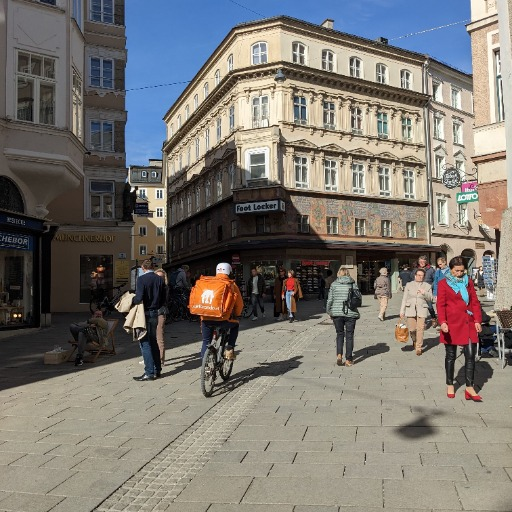
\includegraphics[width=0.8\textwidth]{images/base_image_Salzburg.jpg}}
    \caption{pic of pipeline}
    \label{fig:simpPipeline}
\end{figure}

Based on the pipeline, a simple frontend based on React and NextJS was developed for the time machine \ref{fig:frontendPre}. The frontend implements everything that is needed for uploading and resizing the image. Additionally, it also contains a repertoire of base prompts based on each year. These base prompts contain standard information for each year like which camera was typically used for the time span. Image interrogation and image generation are handled in the background via the stable diffusion webUI to which the frontend makes API calls.
When both the stable diffusion webUI and the web based frontend are locally hosted on a machine it is possible to upload images to the frontend to generate a new image based on a selected year or a GIF based on the whole year range.

\begin{figure}[htbp]
    \centering\small
    {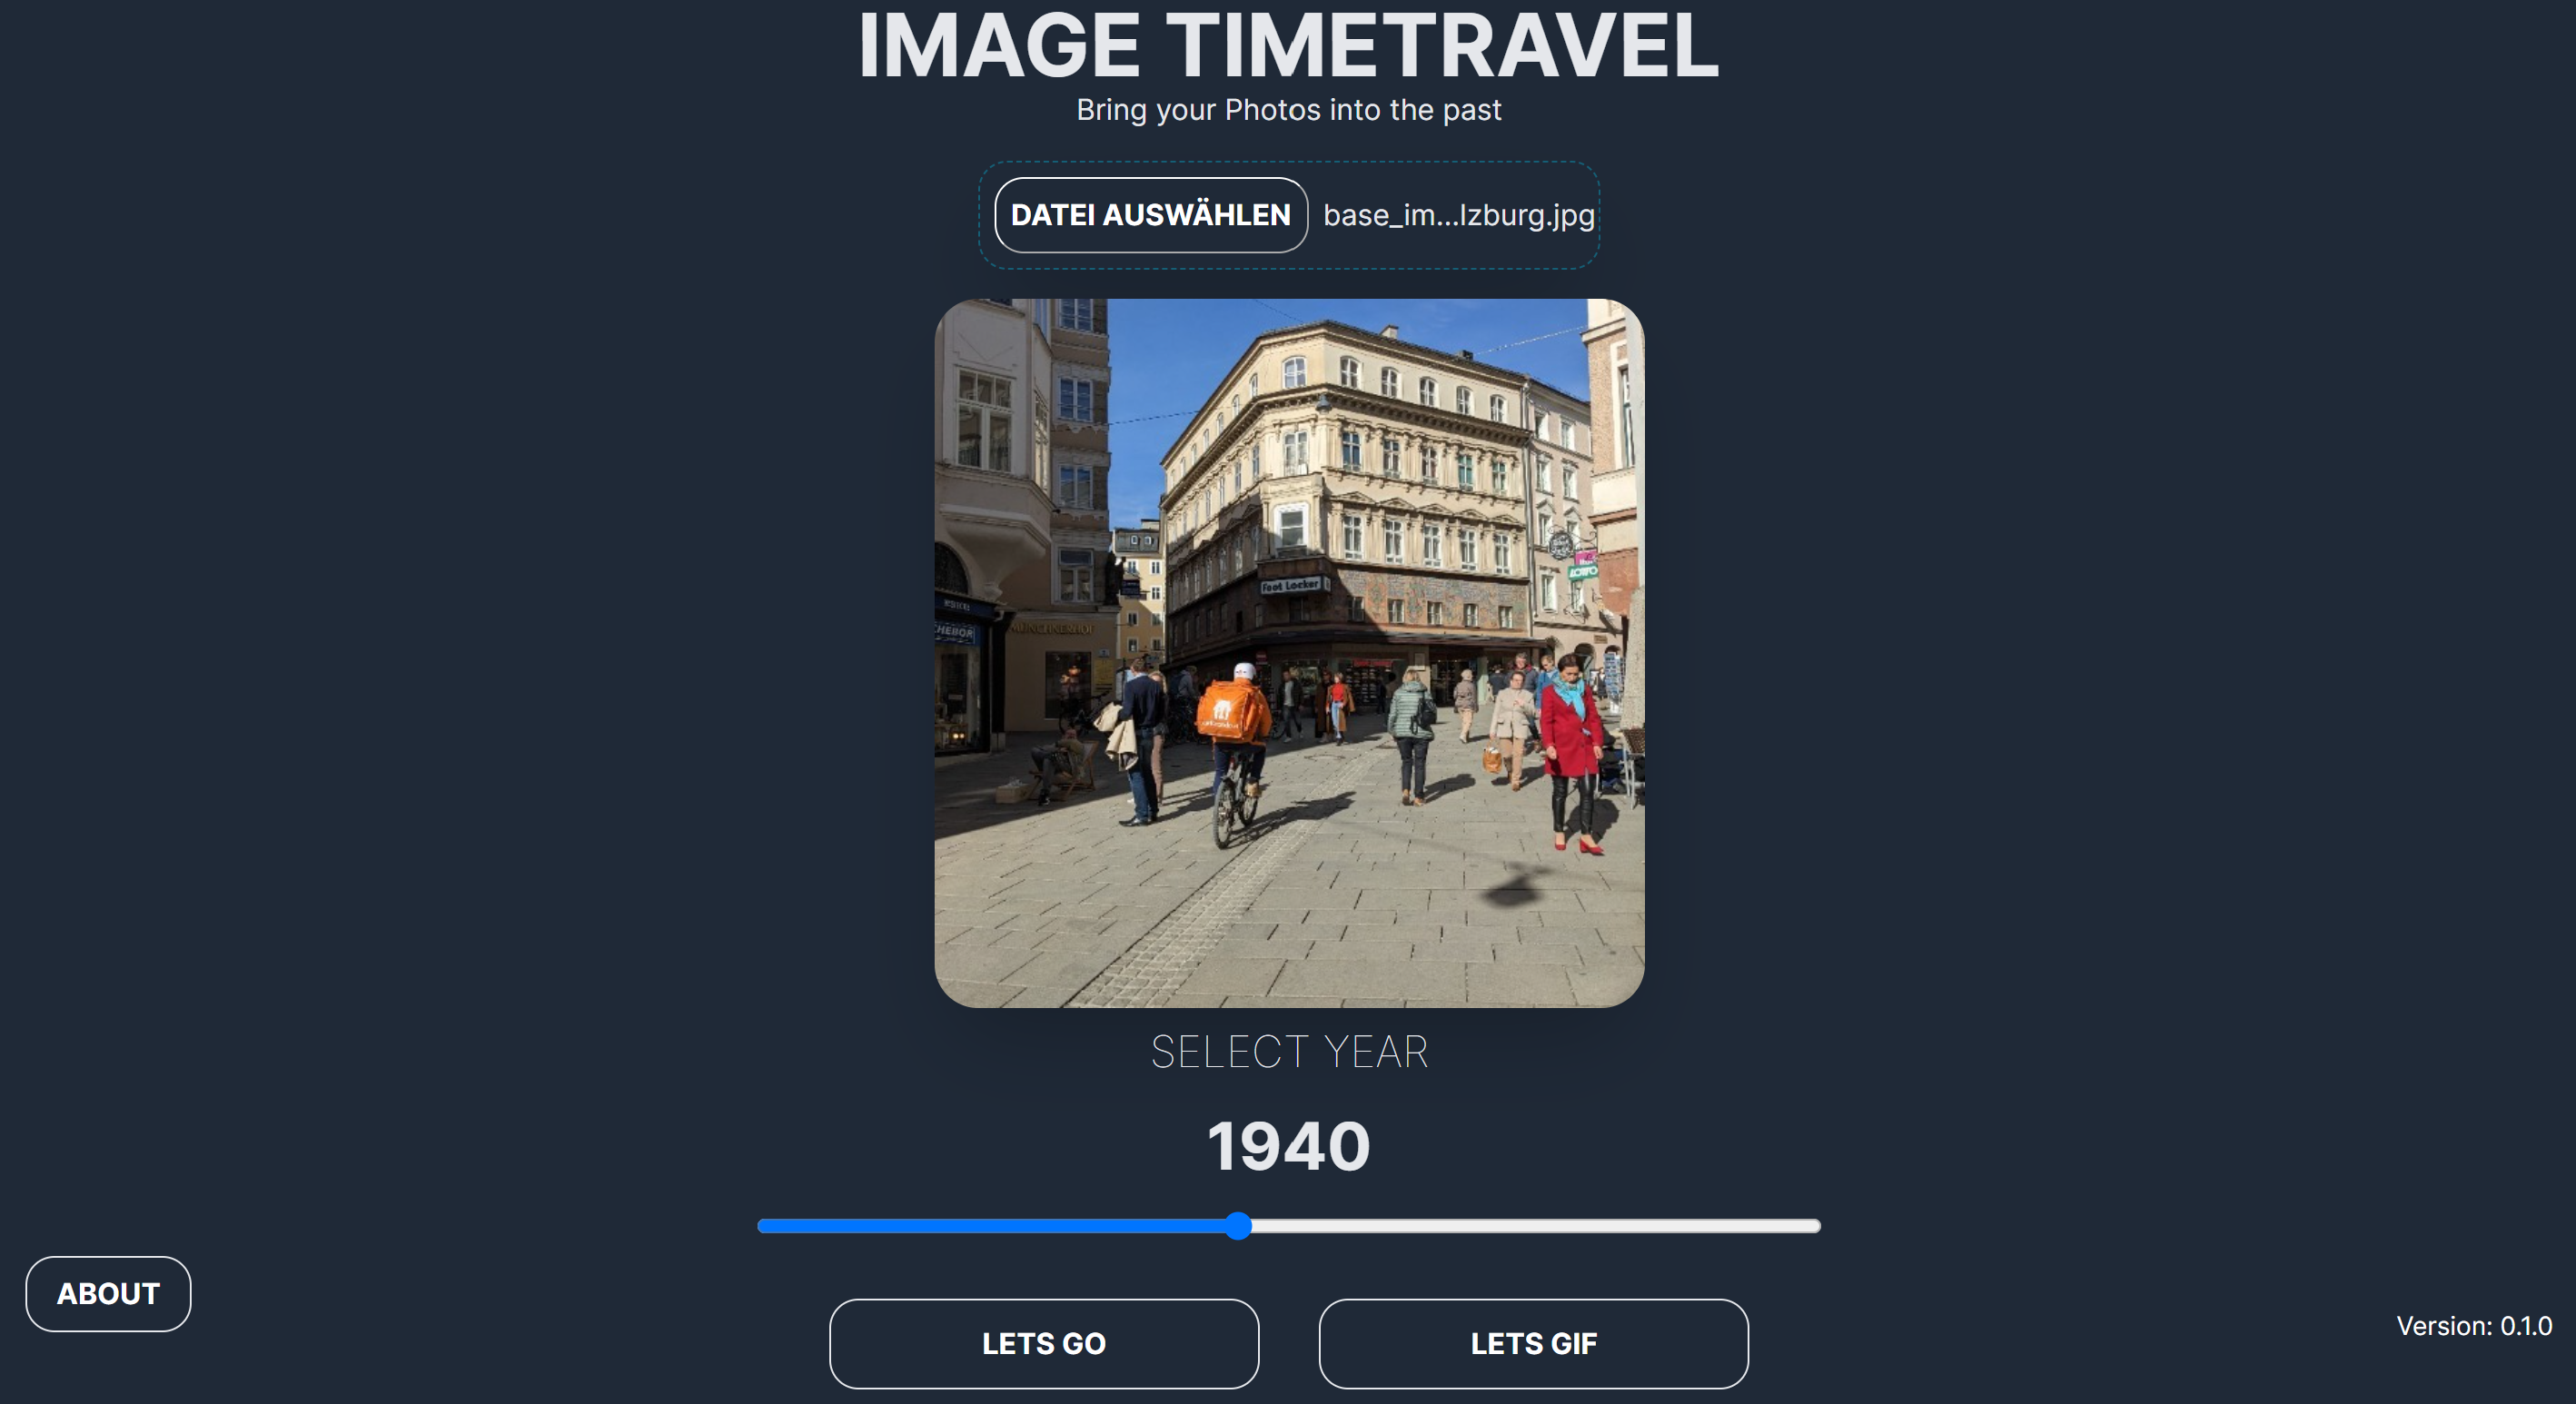
\includegraphics[width=0.8\textwidth]{images/frontendPre.png}}
    \caption{A screenshot of the developed frontend for the time machine. The picture selected is a photograph of a street in Salzburg, Austria taken on a mobile phone}
    \label{fig:frontendPre}
\end{figure}

\begin{figure}[htbp]
    \centering\small
    {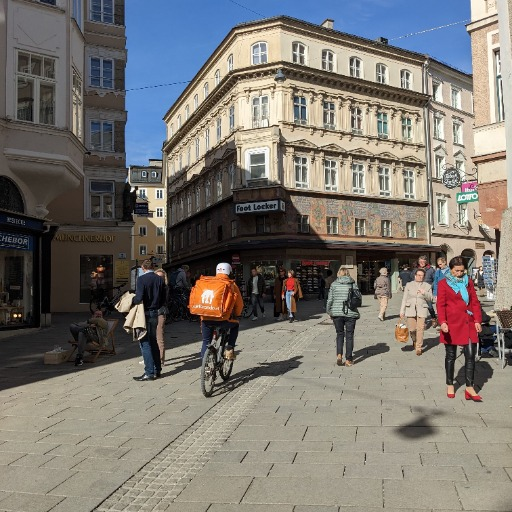
\includegraphics[width=0.8\textwidth]{images/base_image_Salzburg.jpg}}
    \caption{pic of frontend after image generation}
    \label{fig:frontendPost}
\end{figure}

%%%-----------------------------------------------------------------------------
\chapter{System Documentation}
%%%-----------------------------------------------------------------------------
\label{systemDocu}
In this chapter each part of the image generation is explained in detail.

\section{Stable Diffusion Setup}
The stable diffusion webUI \cite{webui} is locally hosted on a machine so that it can be used to transform images. A couple of changes were made the UI to make it possible to generate past version of images.
The specific stable diffusion model used is realistic vision V2.0 \cite{realisticVision}, which is supposed to generate more realistic looking images compared to the base stable diffusion model included in the webUI.

Additionally, the ControlNet plugin \cite{controllNet} is used to enhance images further. With the help of ControlNet canny it is possible to trace the outlines of objects in images that are put into stable diffusion, thereby resulting in images which more closely resemble the original.
Furthermore, the following settings were changed inside the webUI:
\begin{enumerate}
    \item under ControlNet: Allow other script to control this extension
    \item under Interrogate Options: Increase the minimum and maximum description length
\end{enumerate}

Finally, the command line section of the webui-user.bat file inside the folder for the stable diffusion webUI was changed to allow for API calls from the locally hosted front end as can be seen in the following code:

\begin{verbatim}
    set COMMANDLINE_ARGS= --xformers --autolaunch --medvram --api 
    --cors-allow-origins=http://127.0.0.1:7860 --cors-allow-origins=http://localhost:3000
\end{verbatim}

\section{The Frontend}
Give a well-structured description of the architecture and the technical design
of your implementation with sufficient granularity to enable an external person
to continue working on the project.

%%%-----------------------------------------------------------------------------
\chapter{Summary}
%%%-----------------------------------------------------------------------------

Give a concise (and honest) summary of what has been accomplished and what not. 
Point out issues that may warrant further investigation.

%%%-----------------------------------------------------------------------------
\appendix                                                   % Switch to appendix
%%%-----------------------------------------------------------------------------


%%%-----------------------------------------------------------------------------
\MakeBibliography[nosplit]
%%%-----------------------------------------------------------------------------

%%%-----------------------------------------------------------------------------
\end{document}
%%%-----------------------------------------------------------------------------
